\thispagestyle{empty} % supress headers and footers for this page only
\begin{tikzpicture}[remember picture,overlay]

    % \node[opacity=1,inner sep=0pt] at (8.5,-11){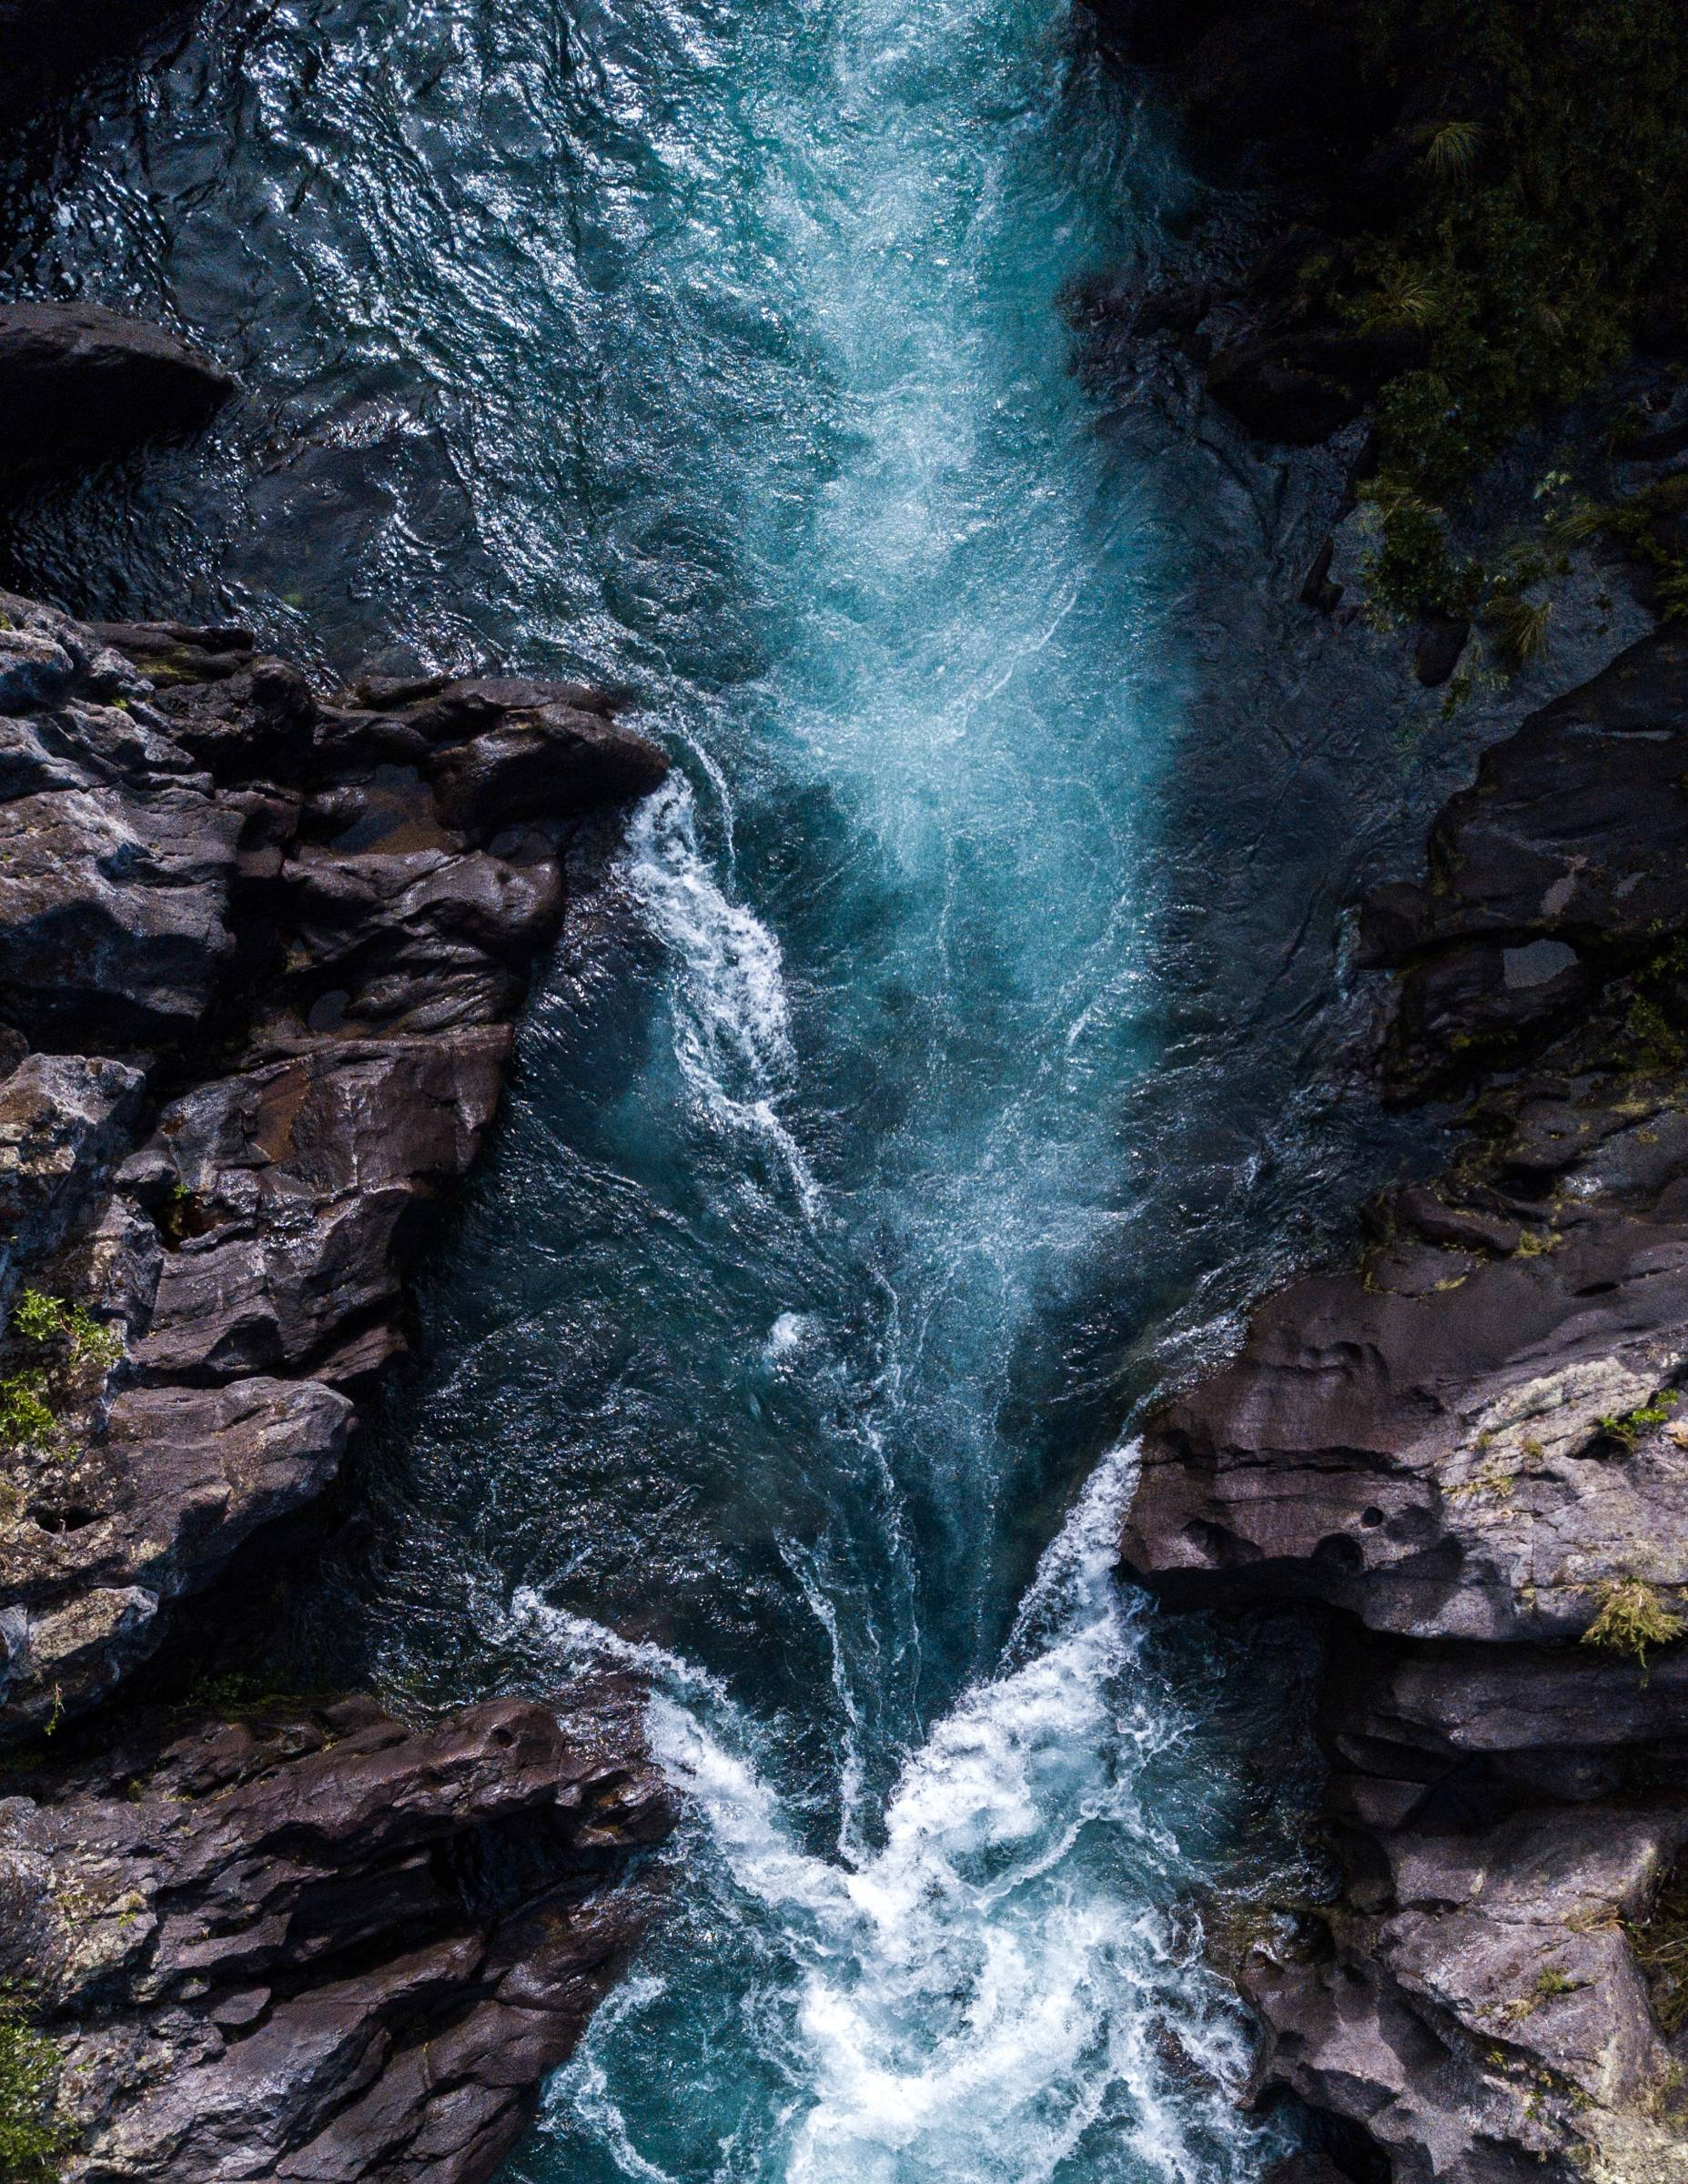
\includegraphics[width=1.08\paperwidth,height=1.05\paperheight]{202402/Exam1/JV_unsplash.jpg}};
    \node[opacity=1,inner sep=0pt] at (8.5,-11){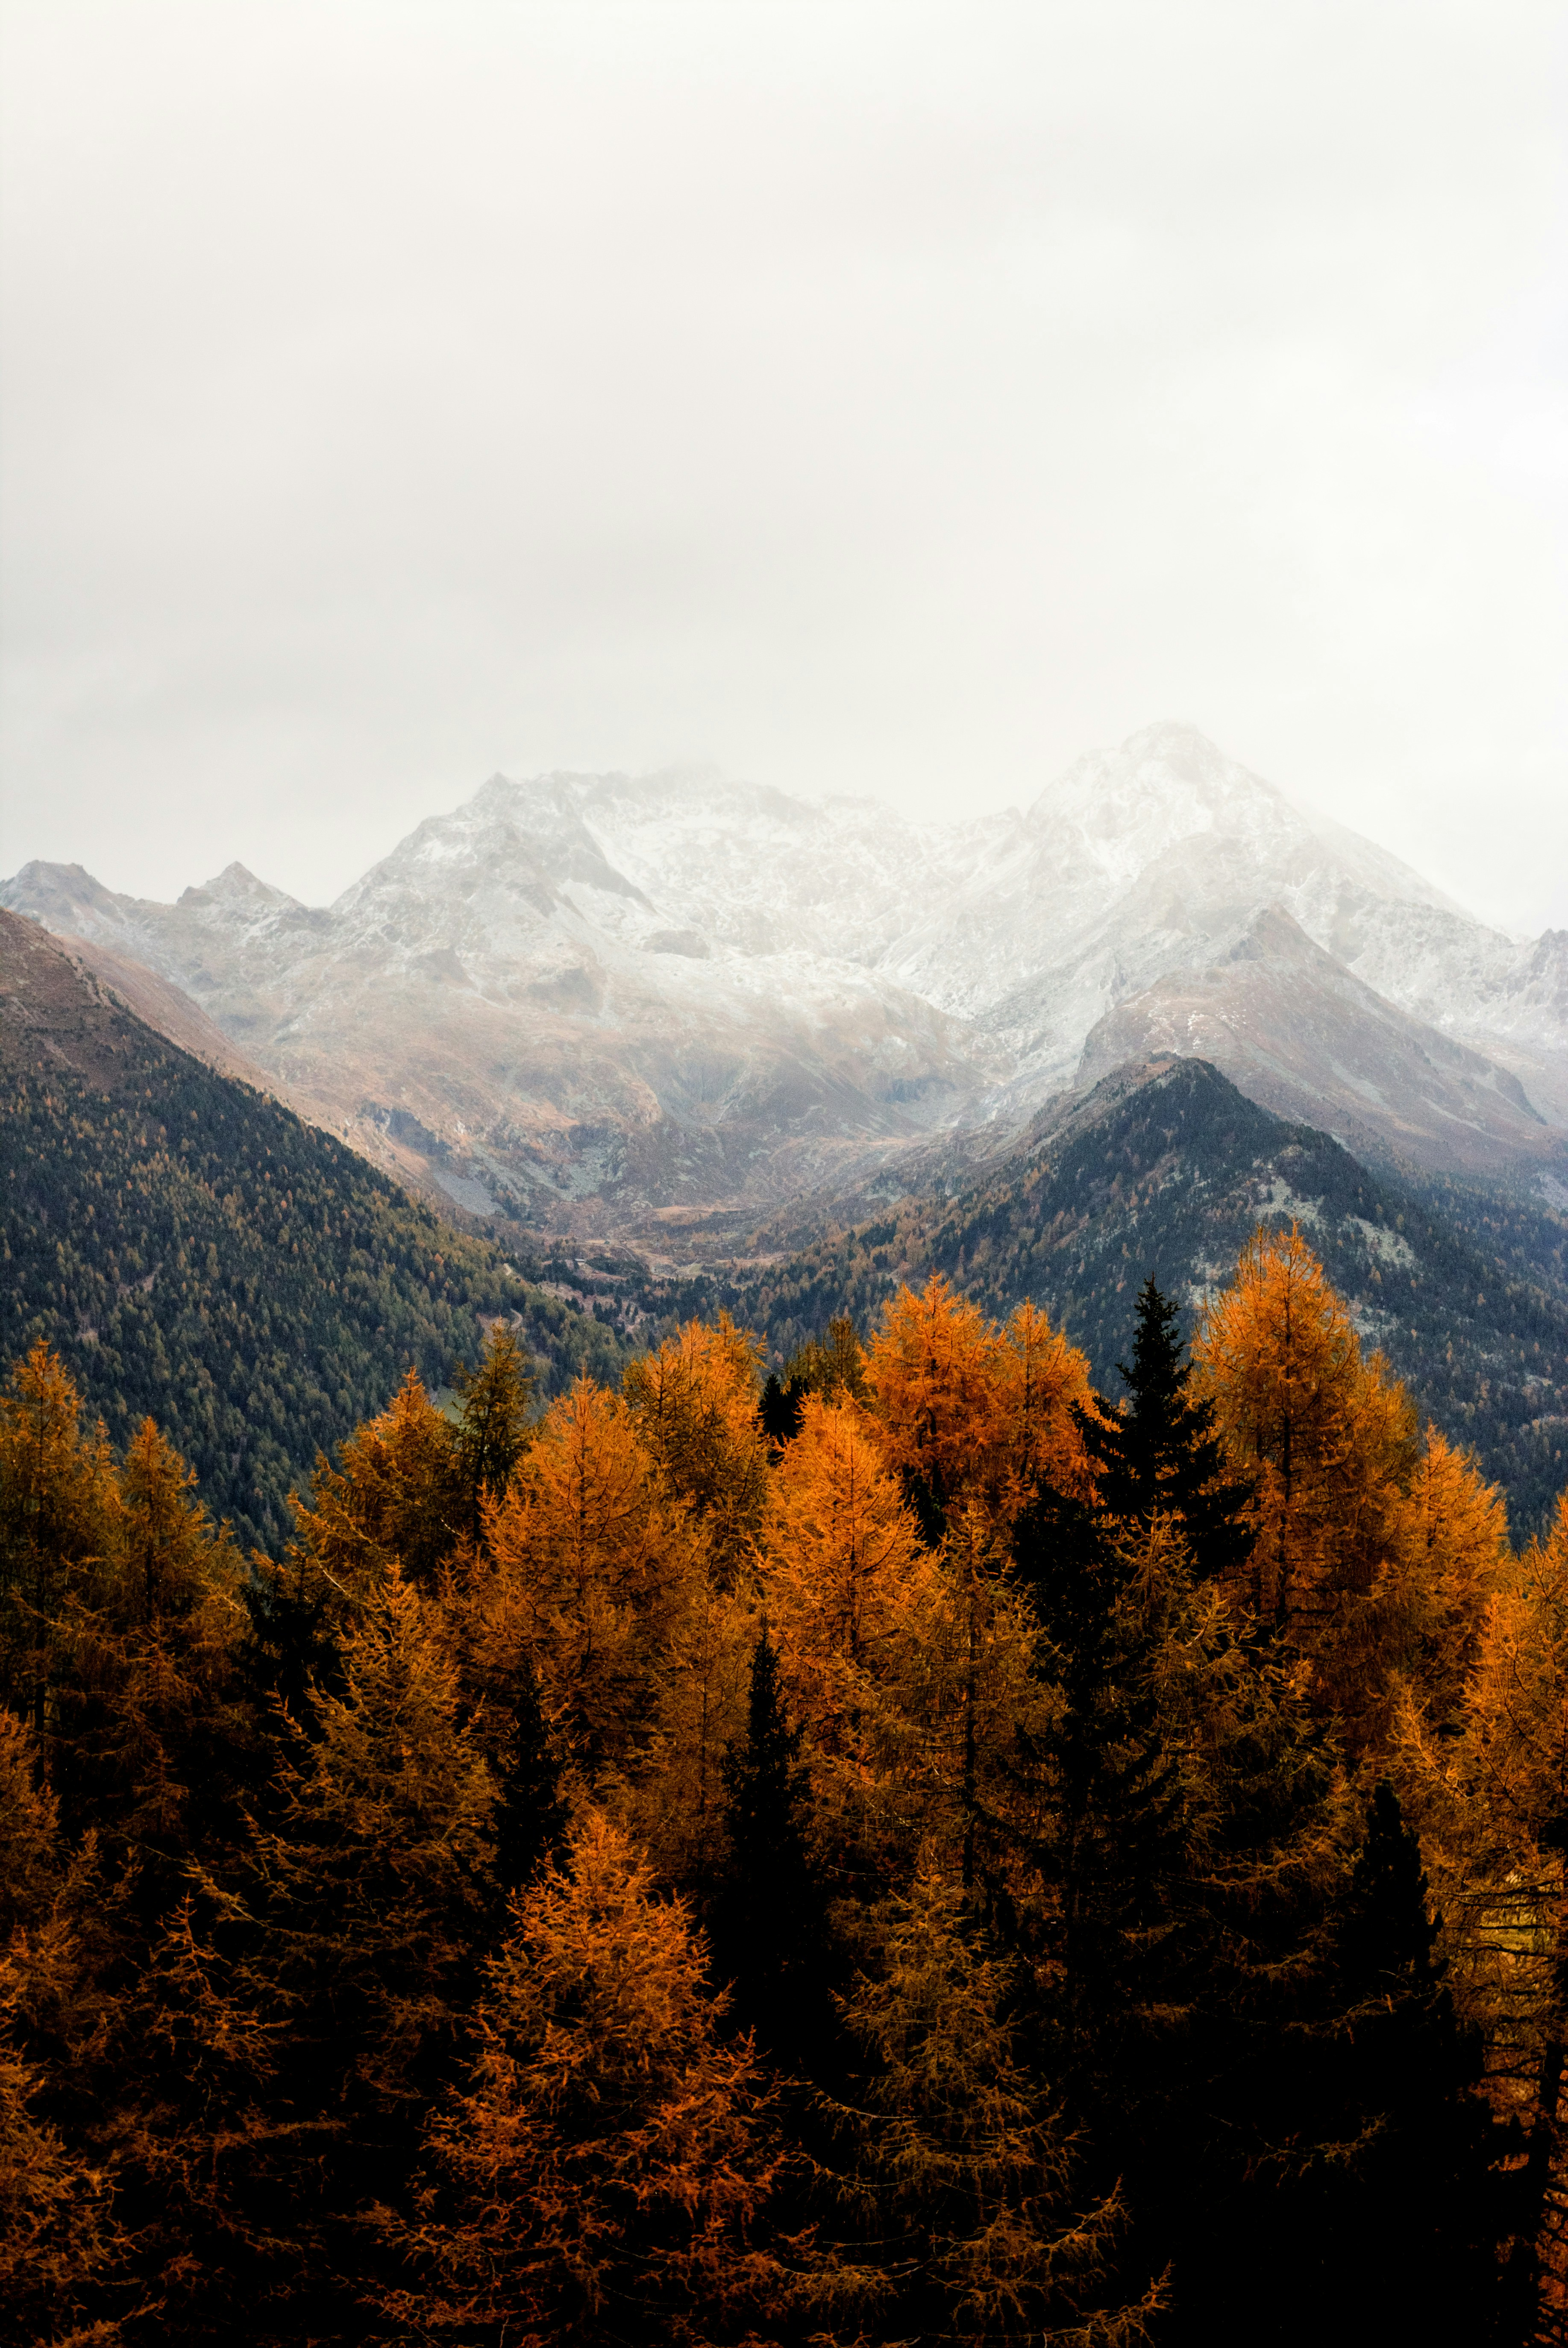
\includegraphics[width=1.08\paperwidth,height=1.05\paperheight]{202402/CoverImages/Cover_eberhard-grossgasteiger-5P91SF0zNsI-unsplash.jpg}};
    
    % \node[opacity=1,inner sep=0pt] at (7.85,-5.75){\includegraphics[width=1.08\paperwidth,height=1.05\paperheight]{CoverImages/drgregmayer_abstract_background_with_cubic_structure_gold_and_n_08699d6c-a73d-4581-8f2b-1f78b8a9e593.png}};
    % \filldraw[black, opacity = 0.65] (-3, 1.25) rectangle (\paperwidth, 7.15);
    % \filldraw[black, opacity = 0.65] (-3, 1.25) rectangle (\paperwidth, 1.15);
    % \filldraw[black, opacity = 0.65] (-3, 1.25) rectangle (\paperwidth, 1.15);
    \draw[] (.02,-0.3) node[right]{\begingroup{\fontfamily{qhv} \fontsize{28pt}{12pt}\selectfont{\color{black} Exam 1}}\endgroup};
    \draw[] (.2,-1.6) node[right]{{\fontfamily{qhv}\selectfont {\Large \color{black} Multivariable Calculus }}};
    \draw[] (.2,-2.4) node[right]{{\fontfamily{qhv}\selectfont {\Large \color{black} MATH 2551 QH }}};        
    \draw[] (.2,-3.2) node[right]{{\fontfamily{qhv}\selectfont {\Large \color{black} Distance Math Program}}};        
    \draw[] (.2,-4.0) node[right]{{\fontfamily{qhv}\selectfont {\Large \color{black} Spring 2024 }}};        

\ifnum \Solutions=1
    \draw[] (.2,-4.8) node[right]{{\fontfamily{qhv}\selectfont {\Large \color{black} Exams with Solutions }}};        
\fi

\end{tikzpicture}